\chaptercustom{4}{KẾT QUẢ MÔ PHỎNG VÀ THẢO LUẬN}
\setcounter{section}{4}
\label{chap:simulation_results}

\subsection{Nguồn dữ liệu và phạm vi đánh giá}
\label{subsec:ch4_data_scope}

Chương này đánh giá kết quả của quy trình mô phỏng đã trình bày ở Chương 3. Phần trình bày lần lượt trả lời ba câu hỏi: kênh tái tạo có giữ được dạng biến thiên của kênh SoCE hay không; sai số giữa các nhánh khác nhau như thế nào; và chi phí thời gian quan sát được trong lần chạy hiện tại là bao nhiêu. Các nhận xét định lượng chỉ dựa trên các hình và bảng kết quả đã được kiểm chứng.

Trong mô phỏng này, SoCE được dùng làm kênh tham chiếu vì nó tính trực tiếp đóng góp của từng MPC tại từng mẫu. Ba nhánh được so sánh với tham chiếu gồm DPS chính xác, DPS xấp xỉ 4D và phương pháp hybrid. Vì cả bốn nhánh dùng cùng một tập MPC, sai khác ở đầu ra xuất phát từ cách tính hệ số và tái tạo kênh, không phải từ một kịch bản truyền sóng khác. Việc đánh giá bắt đầu bằng quan sát định tính trên đáp ứng kênh, sau đó mới dùng chỉ tiêu sai số để định lượng mức sai khác.

Bảng~\ref{tab:ch4_simulation_config} tóm tắt cấu hình mô phỏng dùng cho phần đánh giá. Trong đó, \(M,Q\) xác định số mẫu thời gian và tần số; \(N_{\mathrm{Tx}},N_{\mathrm{Rx}}\) xác định kích thước mảng anten; \(P\) là số MPC; còn \(D_t,D_f,D_{\mathrm{Tx}},D_{\mathrm{Rx}}\) là số véc-tơ DPS được giữ lại ở bốn chiều. Các hệ số \(r\) biểu thị độ phân giải của cơ sở dùng khi xấp xỉ hệ số DPS, không phải số mẫu của khối kênh.

\begin{table}[H]
    \centering
    \small
    \caption{Cấu hình mô phỏng dùng cho kết quả Chương 4}
    \label{tab:ch4_simulation_config}
    \begin{tabular}{ll}
        \toprule
        Tham số & Giá trị \\
        \midrule
        \(M,Q,N_{\mathrm{Tx}},N_{\mathrm{Rx}}\) & \(256,64,4,4\) \\
        \(P\) & \(80\) MPC \\
        \(D_t,D_f,D_{\mathrm{Tx}},D_{\mathrm{Rx}}\) & \(6,9,4,4\) \\
        \(D_{\mathrm{total}}\) & \(864\) \\
        \(r_t,r_f,r_{\mathrm{Tx}},r_{\mathrm{Rx}}\) & \(2,512,512,512\) \\
        \(\nu_{\mathrm{D,max}}\) & \(4{,}8225\times10^{-5}\) \\
        \(\theta_{\max}\) & \(5{,}55\times10^{-2}\) \\
        \bottomrule
    \end{tabular}
\end{table}

\subsection{So sánh đáp ứng kênh}
\label{subsec:ch4_channel_response}

Trước hết, cần kiểm tra liệu phương pháp tái tạo có giữ được cấu trúc chung của đáp ứng kênh hay không. Hình~\ref{fig:mimo_dps_kaltenberger_approx_tx1_rx1} minh họa biên độ đáp ứng của cặp anten phát--thu thứ nhất. Trục \(m\) biểu diễn chỉ số mẫu thời gian, trục \(q\) biểu diễn chỉ số điểm tần số, còn màu sắc biểu diễn độ lớn của hệ số kênh phức. Bốn ô lần lượt thể hiện SoCE tham chiếu, DPS chính xác, phương pháp hybrid và sai số tuyệt đối giữa SoCE với hybrid.

\begin{figure}[H]
    \centering
    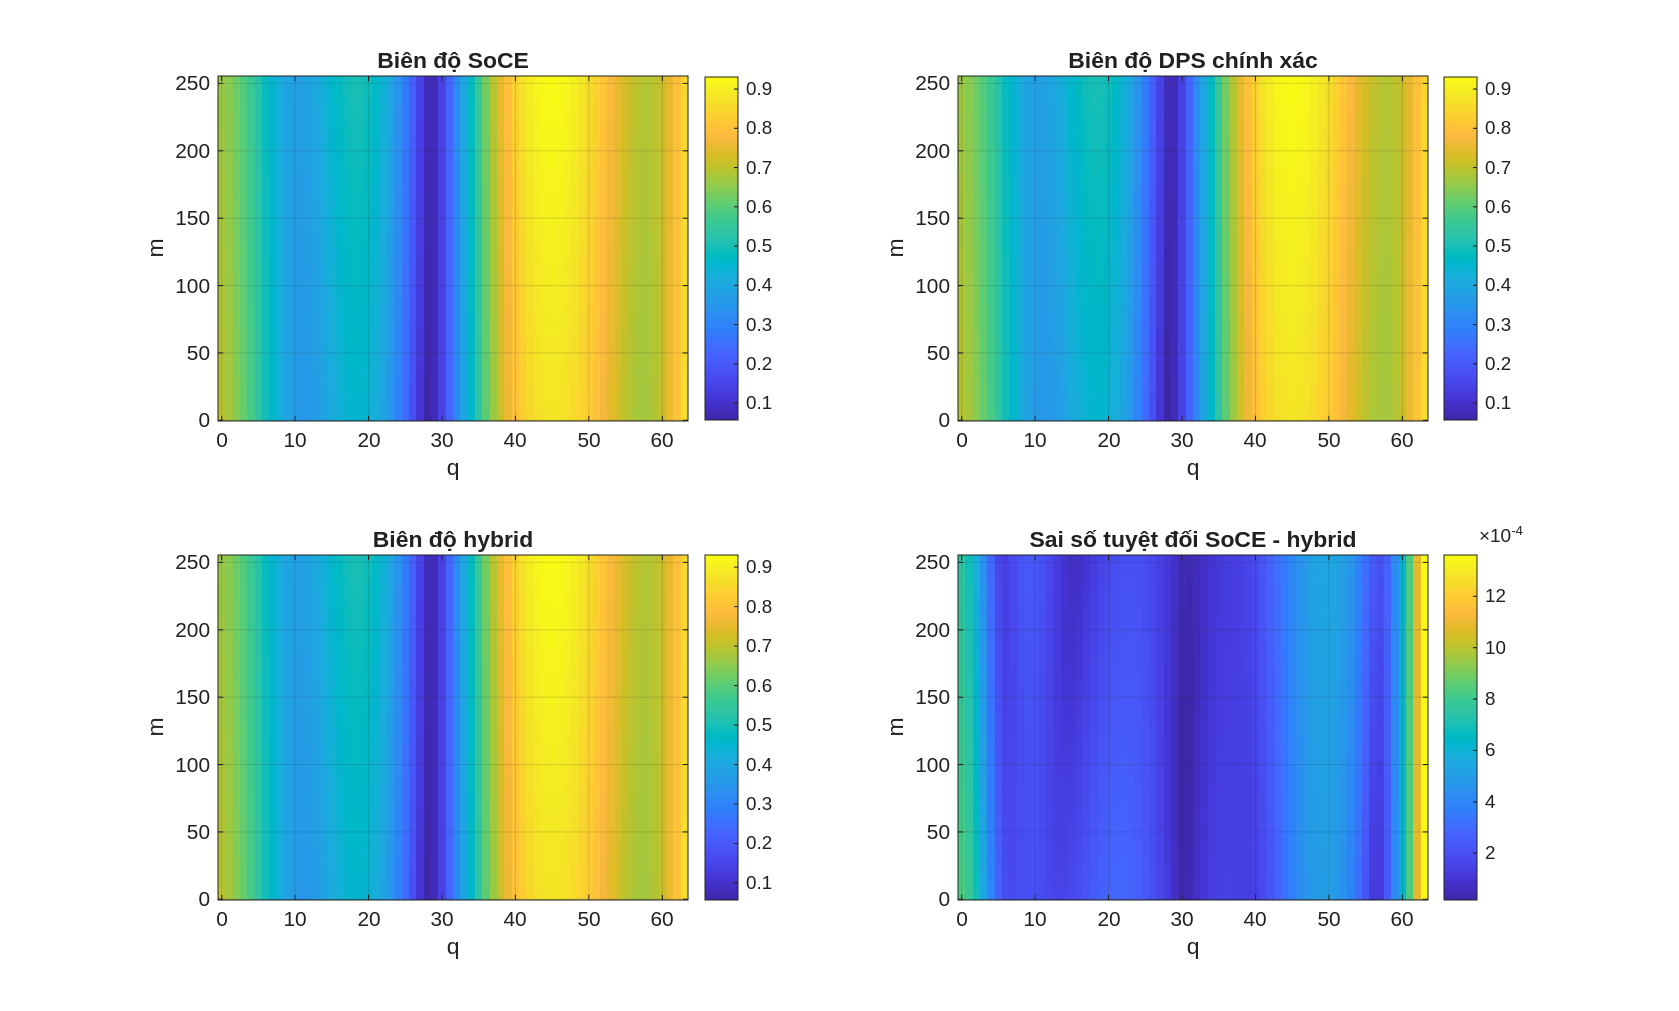
\includegraphics[width=0.9\textwidth]{results/figures/mimo_dps_kaltenberger_approx_tx1_rx1.png}
    \caption{So sánh đáp ứng kênh giữa SoCE, DPS chính xác và phương pháp hybrid cho cặp anten phát--thu thứ nhất}
    \label{fig:mimo_dps_kaltenberger_approx_tx1_rx1}
\end{figure}

Hình~\ref{fig:mimo_dps_kaltenberger_approx_tx1_rx1} cho thấy đáp ứng tái tạo bằng DPS chính xác có dạng biên độ gần với SoCE tham chiếu. Phương pháp hybrid cũng giữ được các vùng biên độ lớn, nhỏ và xu hướng biến thiên theo tần số. Trong cấu hình này, tích \(M\nu_{\mathrm{D,max}}\) nhỏ nên pha Doppler chỉ thay đổi ít trên một khối; vì vậy, biên độ quan sát được biến thiên yếu theo chỉ số thời gian \(m\). Ô sai số tuyệt đối ở góc dưới bên phải giúp xác định vị trí sai khác, nhưng hình ảnh của một cặp anten chưa đủ để đánh giá toàn bộ tensor kênh. Vì vậy, phần tiếp theo sử dụng MSE, NMSE và sai số cực đại được tính trên tất cả mẫu thời gian, tần số và cặp anten.

\subsection{Kết quả sai số và thời gian chạy}
\label{subsec:ch4_error_runtime}

Ba chỉ tiêu sai số cung cấp ba cách nhìn bổ sung. MSE là trung bình bình phương độ lớn sai số trên toàn bộ tensor; sai số tuyệt đối lớn nhất cho biết trường hợp lệch nhiều nhất tại một phần tử; còn NMSE chuẩn hóa MSE theo công suất trung bình của kênh tham chiếu. Nhờ phép chuẩn hóa, NMSE là đại lượng không có đơn vị và thuận tiện để so sánh giữa các nhánh. Với kênh tham chiếu \(H_{\mathrm{SoCE}}\) và kênh tái tạo \(\hat{H}\), NMSE được xác định bởi:
\begin{equation}
\mathrm{NMSE}
=
\frac{\mathbb{E}\{|H_{\mathrm{SoCE}}-\hat{H}|^2\}}
{\mathbb{E}\{|H_{\mathrm{SoCE}}|^2\}}.
\label{eq:ch4_nmse_definition}
\end{equation}
Trong \eqref{eq:ch4_nmse_definition}, ký hiệu \(\mathbb{E}\{\cdot\}\) là phép lấy trung bình trên toàn bộ phần tử của khối kênh mô phỏng, không phải trung bình của nhiều lần sinh kênh độc lập. Giá trị NMSE càng gần không thì kênh tái tạo càng gần SoCE theo nghĩa năng lượng sai số.

Hình~\ref{fig:mimo_dps_kaltenberger_approx_nmse_bar} biểu diễn NMSE của ba nhánh DPS theo thang logarit. Trên thang này, mỗi khoảng cách một bậc tương ứng với hệ số mười; do đó, biểu đồ cho phép quan sát rõ các giá trị sai số chênh nhau nhiều bậc độ lớn.

\begin{figure}[H]
    \centering
    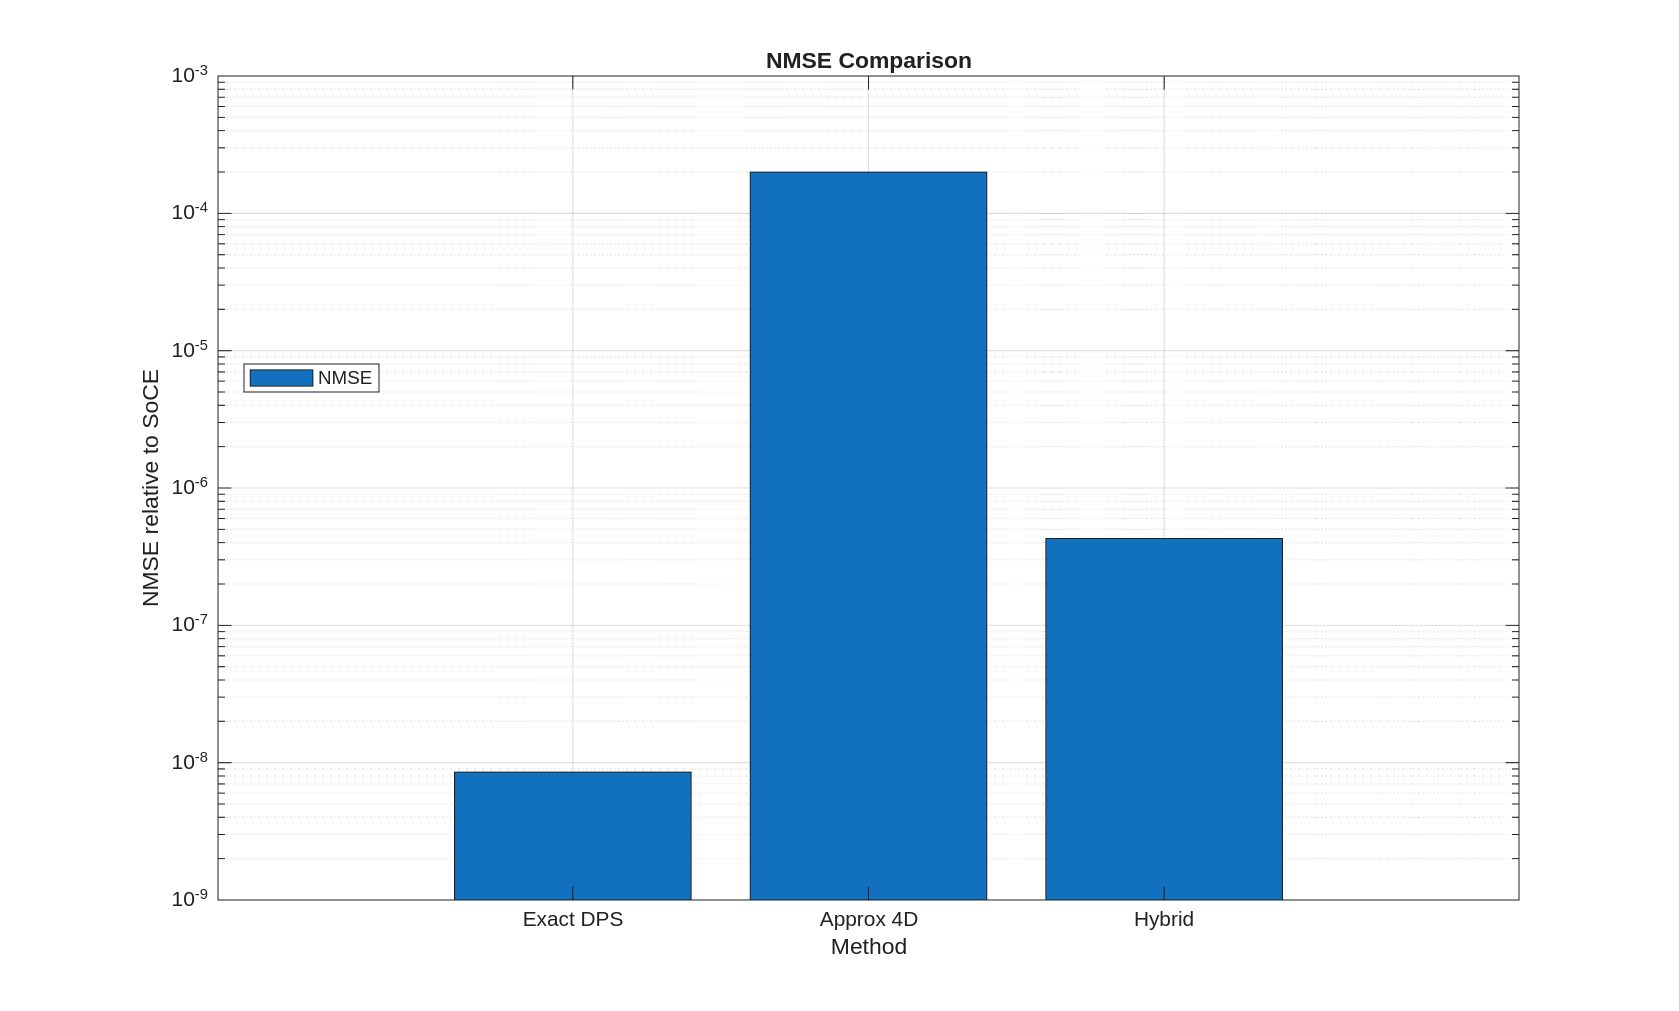
\includegraphics[width=0.9\textwidth]{results/figures/mimo_dps_kaltenberger_approx_nmse_bar.png}
    \caption{So sánh NMSE của các nhánh DPS so với kênh SoCE tham chiếu}
    \label{fig:mimo_dps_kaltenberger_approx_nmse_bar}
\end{figure}

Từ Hình~\ref{fig:mimo_dps_kaltenberger_approx_nmse_bar}, nhánh DPS chính xác có NMSE nhỏ nhất, ở mức \(8{,}53\times10^{-9}\). Nhánh DPS xấp xỉ 4D có NMSE lớn nhất, \(1{,}99\times10^{-4}\). Phương pháp hybrid đạt \(4{,}29\times10^{-7}\), nằm giữa hai nhánh trên nhưng thấp hơn xấp xỉ 4D hơn hai bậc độ lớn. Thứ tự này cho thấy việc tránh xấp xỉ DPS ở hai chiều anten giúp giảm sai số trong cấu hình hiện tại; nguyên nhân của từng nhánh được phân tích riêng ở Mục~\ref{subsec:ch4_branch_discussion}.

Bảng~\ref{tab:ch4_metrics} bổ sung các giá trị MSE, sai số cực đại và hai thành phần thời gian. Cột \(t_{\alpha}\) là thời gian tạo tensor hệ số; cột \(t_{\mathrm{rec}}\) là thời gian tái tạo kênh từ tensor đó. Tổng hai cột là thời gian xử lý của một nhánh DPS sau khi các cơ sở cần thiết đã được tạo.

\begin{table}[H]
    \centering
    \scriptsize
    \setlength{\tabcolsep}{3pt}
    \caption{Sai số và thời gian chạy của các nhánh mô phỏng}
    \label{tab:ch4_metrics}
    \begin{tabularx}{\textwidth}{>{\raggedright\arraybackslash}X c c c c c}
        \toprule
        Nhánh mô phỏng & MSE & NMSE & Max \(|e|\) & \(t_{\alpha}\) (s) & \(t_{\mathrm{rec}}\) (s) \\
        \midrule
        DPS chính xác
        & \(3{,}43\times10^{-9}\)
        & \(8{,}53\times10^{-9}\)
        & \(2{,}01\times10^{-4}\)
        & \(9{,}14\times10^{-3}\)
        & \(8{,}18\times10^{-3}\) \\
        DPS xấp xỉ 4D
        & \(8{,}03\times10^{-5}\)
        & \(1{,}99\times10^{-4}\)
        & \(2{,}23\times10^{-2}\)
        & \(1{,}50\times10^{-2}\)
        & \(6{,}94\times10^{-3}\) \\
        Phương pháp hybrid
        & \(1{,}72\times10^{-7}\)
        & \(4{,}29\times10^{-7}\)
        & \(1{,}67\times10^{-3}\)
        & \(5{,}88\times10^{-3}\)
        & \(1{,}18\times10^{-3}\) \\
        \bottomrule
    \end{tabularx}
\end{table}

Các giá trị trong Bảng~\ref{tab:ch4_metrics} cho thấy MSE, NMSE và sai số tuyệt đối lớn nhất đều xếp ba nhánh theo cùng một thứ tự. Điều này giúp tránh kết luận dựa riêng vào một chỉ tiêu. Về thời gian, nhánh DPS xấp xỉ 4D tốn nhiều thời gian tạo hệ số nhất vì phải xấp xỉ trên cả bốn chiều. Phương pháp hybrid có thời gian tái tạo thấp nhất vì chỉ thực hiện phép tái tạo DPS theo thời gian và tần số; hai chiều anten đã được giữ trực tiếp trong tensor hệ số.

Hình~\ref{fig:mimo_dps_kaltenberger_approx_runtime_bar} so sánh thời gian chạy của SoCE và ba nhánh DPS trong cùng lần mô phỏng. Đối với mỗi nhánh DPS, tổng thời gian gồm thời gian tạo hệ số và thời gian tái tạo trong Bảng~\ref{tab:ch4_metrics}. Thời gian tạo các cơ sở DPS và cơ sở độ phân giải cao được thực hiện trước các lệnh đo thời gian nên chưa được tính trong biểu đồ.

\begin{figure}[H]
    \centering
    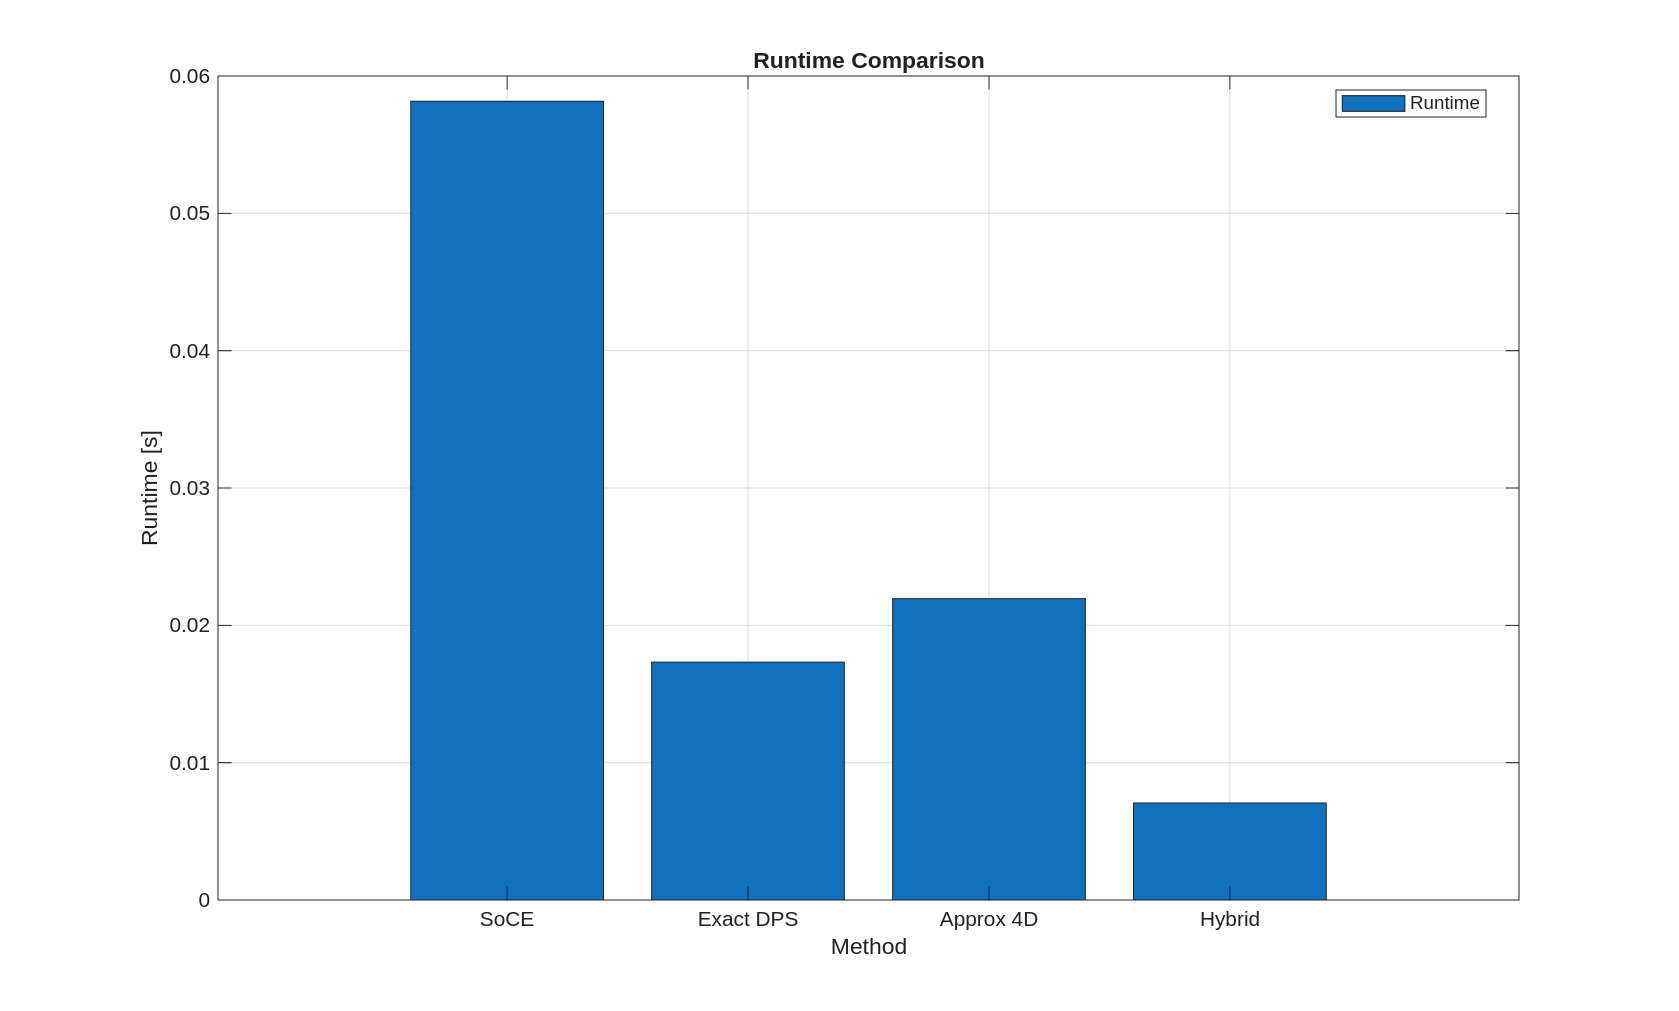
\includegraphics[width=0.9\textwidth]{results/figures/mimo_dps_kaltenberger_approx_runtime_bar.png}
    \caption{So sánh thời gian chạy của SoCE và các nhánh DPS trong cấu hình mô phỏng hiện tại}
    \label{fig:mimo_dps_kaltenberger_approx_runtime_bar}
\end{figure}

Từ Hình~\ref{fig:mimo_dps_kaltenberger_approx_runtime_bar}, thời gian tính SoCE tham chiếu trong lần chạy này là \(0{,}058161\,\mathrm{s}\). Tổng thời gian tạo hệ số và tái tạo của DPS chính xác là khoảng \(0{,}017324\,\mathrm{s}\), của DPS xấp xỉ 4D là khoảng \(0{,}021947\,\mathrm{s}\), và của phương pháp hybrid là khoảng \(0{,}007063\,\mathrm{s}\). Trong phạm vi phép đo này, cả ba tổng thời gian đều nhỏ hơn thời gian SoCE và hybrid có tổng thời gian thấp nhất. Tuy nhiên, kết quả chưa bao gồm chi phí tạo cơ sở DPS, đồng thời còn phụ thuộc vào máy tính, phiên bản MATLAB, cách véc-tơ hóa và cấp phát bộ nhớ. Vì vậy, các số đo chỉ dùng để so sánh các nhánh trong cùng điều kiện chạy, không phải bảo đảm về tốc độ cho mọi cấu hình.

\subsection{Thảo luận từng nhánh mô phỏng}
\label{subsec:ch4_branch_discussion}

Nhánh DPS chính xác trả lời câu hỏi liệu không gian con đã chọn có đủ để chứa phần lớn năng lượng kênh hay không. NMSE \(8{,}53\times10^{-9}\) cho thấy, với \(D_t=6\), \(D_f=9\), \(D_{\mathrm{Tx}}=4\) và \(D_{\mathrm{Rx}}=4\), sai số cắt không gian con ở mức thấp trong cấu hình hiện tại. Kết quả này không có nghĩa DPS tái tạo chính xác tuyệt đối, mà cho thấy phép chiếu chính xác lên số véc-tơ đang giữ gần với SoCE.

Nhánh DPS xấp xỉ 4D trả lời câu hỏi điều gì xảy ra khi không tính các tích vô hướng chính xác. NMSE \(1{,}99\times10^{-4}\) lớn hơn đáng kể so với DPS chính xác vì hệ số được ước lượng từ hàm sóng DPS trên lưới độ phân giải cao. Khi phép xấp xỉ được áp dụng cho cả bốn chiều, sai số hệ số của từng chiều cùng tham gia vào tích tensor. Vì vậy, nhánh này chủ yếu đóng vai trò chẩn đoán ảnh hưởng của công thức xấp xỉ hệ số, chưa phải lựa chọn phù hợp nhất trong cấu hình đang xét.

Phương pháp hybrid trả lời câu hỏi liệu chỉ xấp xỉ hai chiều có kích thước lớn hơn có tạo được cân bằng tốt hơn hay không. Nhánh này đạt NMSE \(4{,}29\times10^{-7}\) so với SoCE và \(4{,}20\times10^{-7}\) so với DPS chính xác. DPS xấp xỉ chỉ được dùng cho thời gian và tần số, còn phần không gian anten được tính trực tiếp bằng hàm mũ. Với \(N_{\mathrm{Tx}}=N_{\mathrm{Rx}}=4\), cách xử lý này tránh sai số xấp xỉ ở hai chiều anten mà vẫn giữ thời gian tái tạo thấp trong phép đo hiện tại. Do đó, hybrid tạo được sự cân bằng phù hợp hơn giữa sai số và thời gian quan sát được trong cấu hình này.

\subsection{Ảnh hưởng của số thành phần đa đường}
\label{subsec:ch4_p_sweep}

Để khảo sát khả năng mở rộng theo số MPC, thí nghiệm quét sử dụng sáu giá trị \(P\in\{10,20,40,80,160,320\}\), trong khi giữ cố định \(M=256\), \(Q=64\), \(N_{\mathrm{Tx}}=N_{\mathrm{Rx}}=4\), \(D_t=6\), \(D_f=9\), \(D_{\mathrm{Tx}}=D_{\mathrm{Rx}}=4\), \(r_t=2\) và \(r_f=512\). Tại mỗi giá trị \(P\), NMSE được đánh giá trên 20 seed. Trong từng seed, các cấu hình dùng chung một tập MPC lồng nhau nhưng trọng số được chuẩn hóa lại theo \(P\) để giữ công suất kỳ vọng xấp xỉ không đổi. Thời gian chạy được đo riêng trên dữ liệu cố định sau bước khởi động, lặp 10 lần và lấy trung vị; thời gian tạo cơ sở DPS không nằm trong phép đo. Thí nghiệm tập trung vào DPS chính xác và phương pháp hybrid vì hai nhánh này lần lượt thể hiện sai số cắt không gian con và phương án xấp xỉ phù hợp hơn cho cấu hình MIMO đang xét.

Hình~\ref{fig:mimo_dps_kaltenberger_p_sweep_nmse} biểu diễn trung vị NMSE và khoảng tứ phân vị từ 20 hiện thực kênh tại mỗi số MPC. Trong toàn bộ dải khảo sát, trung vị NMSE của DPS chính xác nằm trong khoảng từ \(2{,}98\times10^{-9}\) đến \(5{,}90\times10^{-9}\), còn phương pháp hybrid nằm trong khoảng từ \(1{,}67\times10^{-7}\) đến \(2{,}29\times10^{-7}\). Như vậy, thứ tự sai số giữa hai nhánh được duy trì tại cả sáu điểm và trên các khoảng tứ phân vị quan sát được: DPS chính xác có NMSE thấp hơn hybrid trong thí nghiệm này.

\begin{figure}[H]
    \centering
    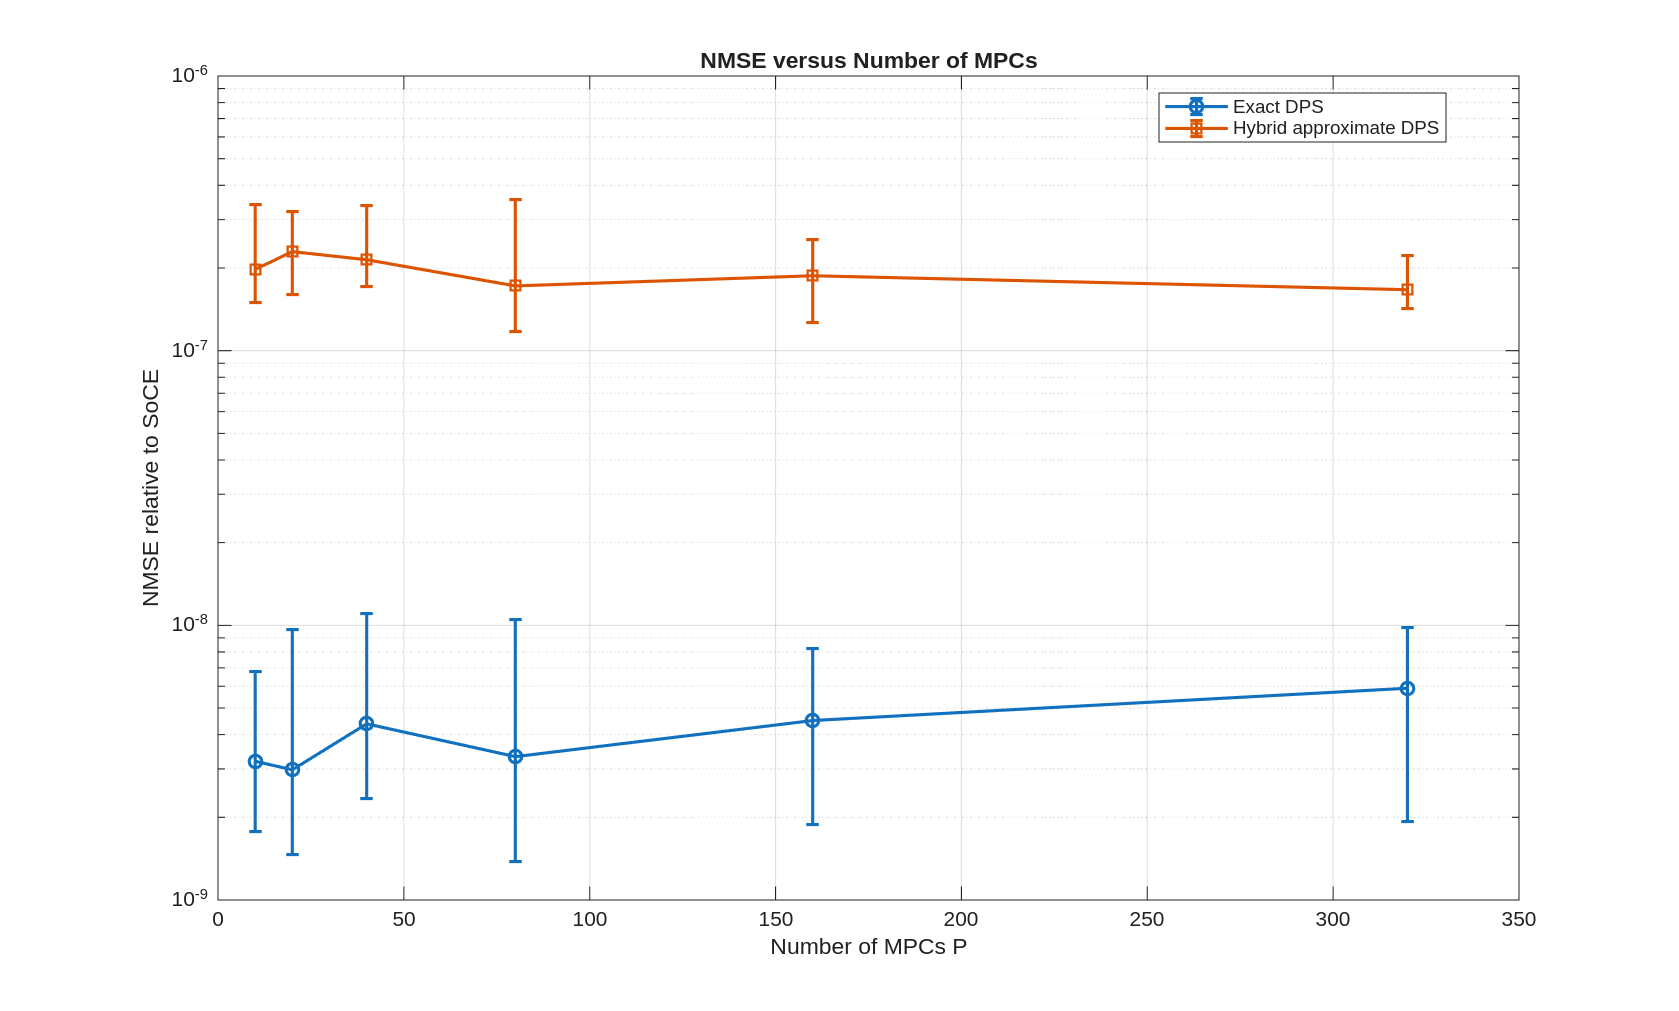
\includegraphics[width=0.9\textwidth]{results/figures/mimo_dps_kaltenberger_p_sweep_nmse.png}
    \caption{NMSE của DPS chính xác và phương pháp hybrid khi thay đổi số MPC}
    \label{fig:mimo_dps_kaltenberger_p_sweep_nmse}
\end{figure}

Các trung vị NMSE không biến thiên đơn điệu theo \(P\), đồng thời các khoảng tứ phân vị của cùng một nhánh chồng lấn đáng kể giữa các giá trị \(P\). Vì NMSE được chuẩn hóa theo công suất của từng kênh tham chiếu và còn phụ thuộc vào vị trí, pha, trọng số MPC, kết quả hiện tại không cho thấy sai số tăng có hệ thống khi số MPC tăng. Kết luận phù hợp trong phạm vi sweep này là số MPC ảnh hưởng ít đến mức NMSE điển hình khi miền giới hạn băng, số chiều DPS và hệ số phân giải được giữ cố định.

Hình~\ref{fig:mimo_dps_kaltenberger_p_sweep_runtime} cho thấy thời gian SoCE tăng rõ khi số MPC lớn. Từ \(P=40\) đến \(P=320\), trung vị thời gian SoCE tăng từ \(0{,}030090\,\mathrm{s}\) lên \(0{,}253762\,\mathrm{s}\). Tại \(P=320\), trung vị tổng thời gian tạo hệ số và tái tạo là \(0{,}015057\,\mathrm{s}\) đối với DPS chính xác và \(0{,}014187\,\mathrm{s}\) đối với hybrid, đều thấp hơn thời gian SoCE trong cùng phép đo. Kết quả này phù hợp với phân tích độ phức tạp: SoCE phải cộng đóng góp của từng MPC trên toàn bộ khối mẫu, trong khi phần tái tạo DPS phụ thuộc chủ yếu vào kích thước cơ sở đã chọn.

\begin{figure}[H]
    \centering
    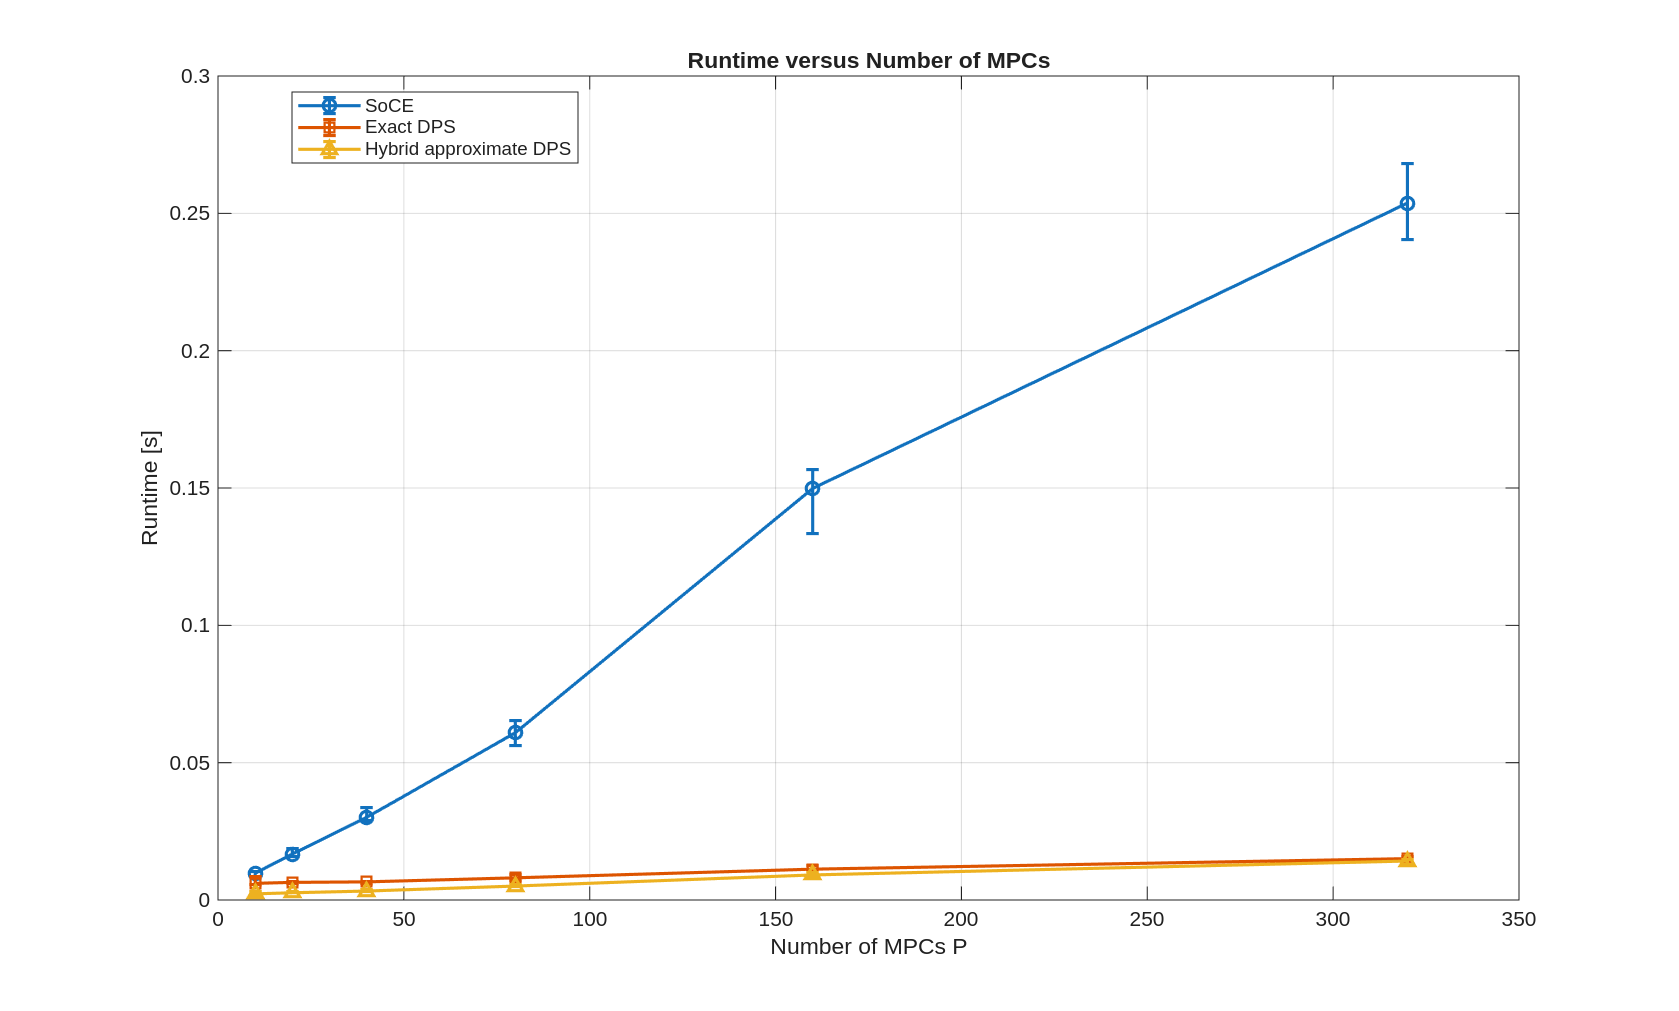
\includegraphics[width=0.9\textwidth]{results/figures/mimo_dps_kaltenberger_p_sweep_runtime.png}
    \caption{Thời gian chạy của SoCE, DPS chính xác và phương pháp hybrid khi thay đổi số MPC}
    \label{fig:mimo_dps_kaltenberger_p_sweep_runtime}
\end{figure}

Các thanh sai số trên Hình~\ref{fig:mimo_dps_kaltenberger_p_sweep_runtime} biểu diễn khoảng tứ phân vị của 10 lần đo. Sau khi có bước khởi động và đo lặp, điểm \(P=10\) không còn biểu hiện thời gian cao bất thường so với các điểm kế tiếp. Tuy nhiên, các số đo vẫn phụ thuộc vào máy tính, phiên bản MATLAB, trạng thái hệ thống và cách triển khai; vì vậy chúng chỉ được dùng để đánh giá xu hướng và so sánh các nhánh trong cùng môi trường thực thi.

\subsection{Benchmark bốn phương pháp và điểm hòa vốn}
\label{subsec:ch4_four_method_benchmark}

Để phân biệt lợi ích do lựa chọn cơ sở với lợi ích do tối ưu cách tạo pha, một benchmark riêng được thực hiện cho bốn phương pháp: SoCE trực tiếp, SoCE đệ quy, CE-BEM và DPS chính xác. Các phương pháp dùng chung khối kênh kích thước \(256\times64\times4\times4\), cùng các tập MPC và cùng số chiều \((6,9,4,4)\) cho hai mô hình khai triển cơ sở. CE-BEM sử dụng các hàm mũ có tần số phân bố đều trong từng miền giới hạn băng và hệ số bình phương tối thiểu; DPS dùng phép chiếu chính xác. Cách thiết lập này giúp so sánh hai cơ sở mà không trộn thêm sai số của công thức hệ số DPS xấp xỉ.

NMSE được tổng hợp trên 20 hiện thực kênh tại mỗi giá trị \(P\), còn thời gian được đo 10 lần trên dữ liệu cố định sau bước khởi động và lấy trung vị. Thời gian xử lý mỗi khối bao gồm bước tạo hệ số và tái tạo, nhưng không gồm bước tạo cơ sở dùng lại. Hình~\ref{fig:ch4_four_method_runtime} cho thấy chi phí của hai nhánh SoCE tăng rõ theo số MPC, trong khi thời gian của CE-BEM và DPS tăng chậm hơn trong dải khảo sát.

\begin{figure}[H]
    \centering
    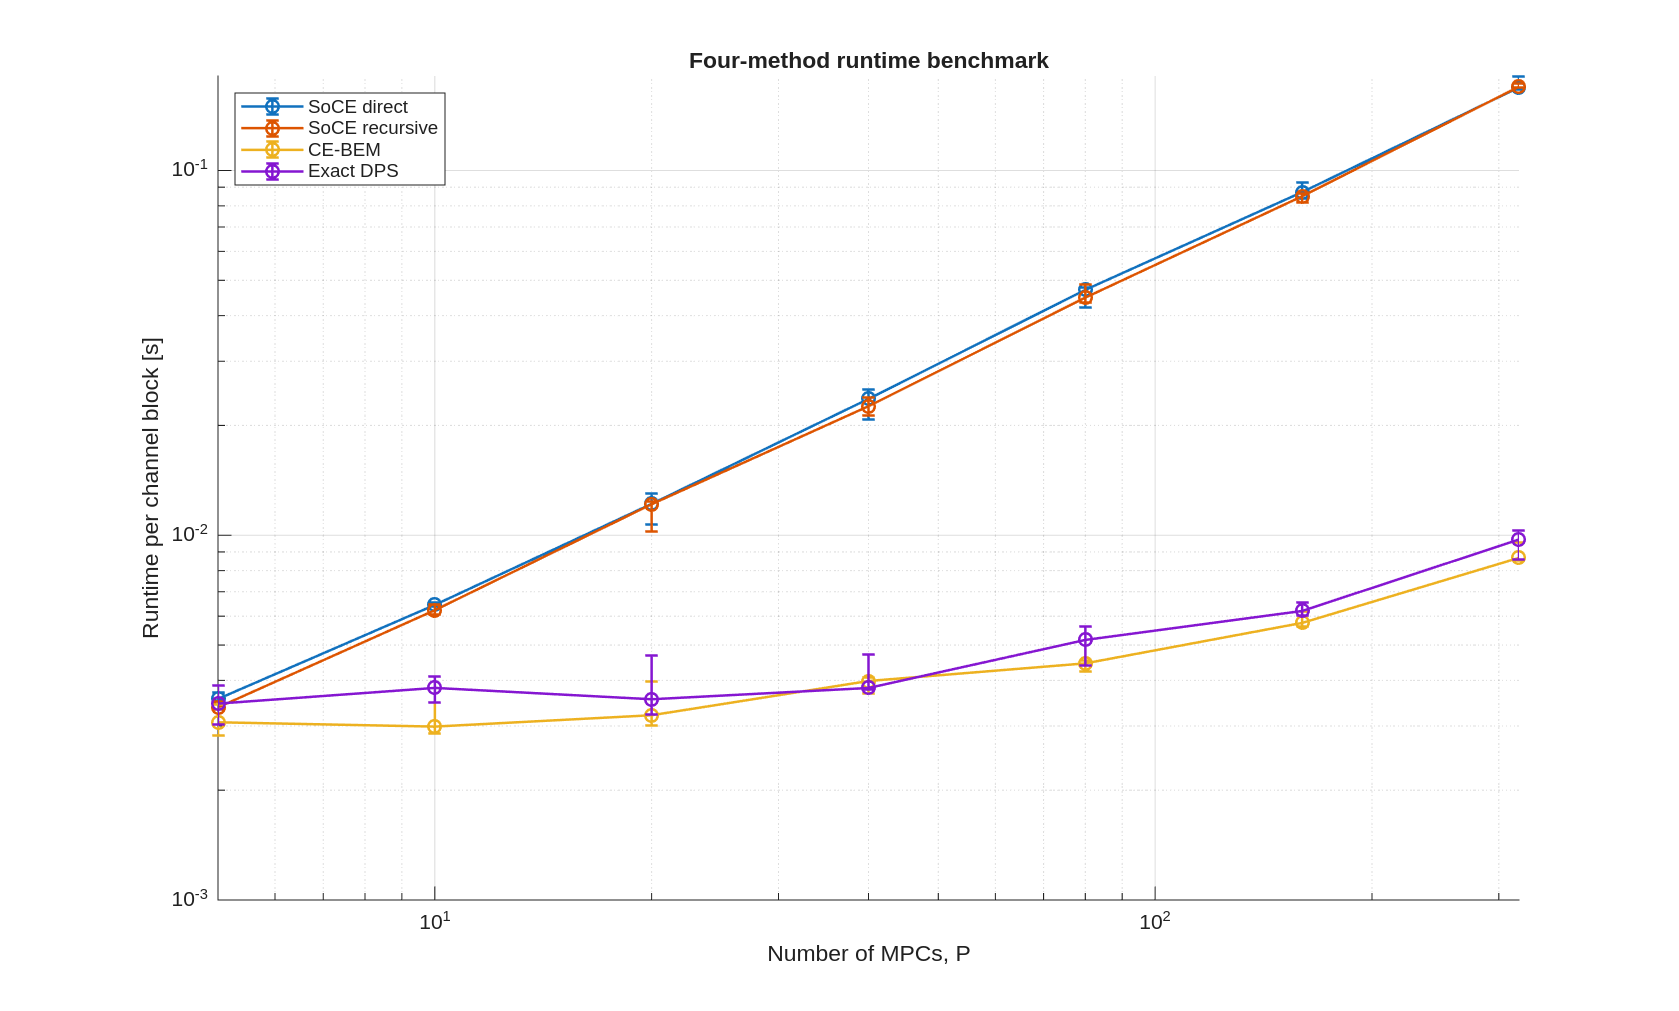
\includegraphics[width=0.9\textwidth]{results/figures/mimo_four_method_benchmark_runtime.png}
    \caption{Thời gian xử lý mỗi khối của bốn phương pháp khi thay đổi số MPC}
    \label{fig:ch4_four_method_runtime}
\end{figure}

Tại \(P=80\), Bảng~\ref{tab:ch4_four_method_p80} cho thấy SoCE đệ quy có thời gian gần SoCE trực tiếp và các khoảng tứ phân vị còn chồng lấn. Do đó, phép cập nhật pha đệ quy không tạo ra lợi thế thời gian rõ ràng trong cách cài đặt MATLAB hiện tại, dù NMSE của nó chỉ ở mức sai số làm tròn. CE-BEM và DPS chính xác lần lượt đạt hệ số tăng tốc khoảng \(10{,}57\) và \(9{,}12\) so với SoCE trực tiếp. DPS có NMSE trung vị thấp hơn CE-BEM gần một bậc độ lớn, lần lượt là \(3{,}33\times10^{-9}\) và \(2{,}96\times10^{-8}\). Kết quả không khẳng định CE-BEM luôn nhanh hơn DPS, vì thời gian còn phụ thuộc cách chọn cơ sở, phép nhân ma trận và khả năng khai thác FFT.

\begin{table}[H]
    \centering
    \small
    \caption{Benchmark bốn phương pháp tại \(P=80\)}
    \label{tab:ch4_four_method_p80}
    \begin{tabular}{lccc}
        \toprule
        Phương pháp & Thời gian trung vị (s) & NMSE trung vị & Tăng tốc ($\times$) \\
        \midrule
        SoCE trực tiếp & \(4{,}708\times10^{-2}\) & \(0\) & \(1{,}00\) \\
        SoCE đệ quy & \(4{,}482\times10^{-2}\) & \(3{,}05\times10^{-29}\) & \(1{,}05\) \\
        CE-BEM & \(4{,}454\times10^{-3}\) & \(2{,}96\times10^{-8}\) & \(10{,}57\) \\
        DPS chính xác & \(5{,}164\times10^{-3}\) & \(3{,}33\times10^{-9}\) & \(9{,}12\) \\
        \bottomrule
    \end{tabular}
\end{table}

Hình~\ref{fig:ch4_four_method_nmse} xác nhận thứ tự sai số của hai mô hình khai triển cơ sở được duy trì trên dải \(P=5\)--\(320\). NMSE không tăng đơn điệu theo \(P\), phù hợp với việc sai số chủ yếu do mức độ phù hợp của không gian con với vị trí tần số MPC, thay vì chỉ do số lượng MPC.

\begin{figure}[H]
    \centering
    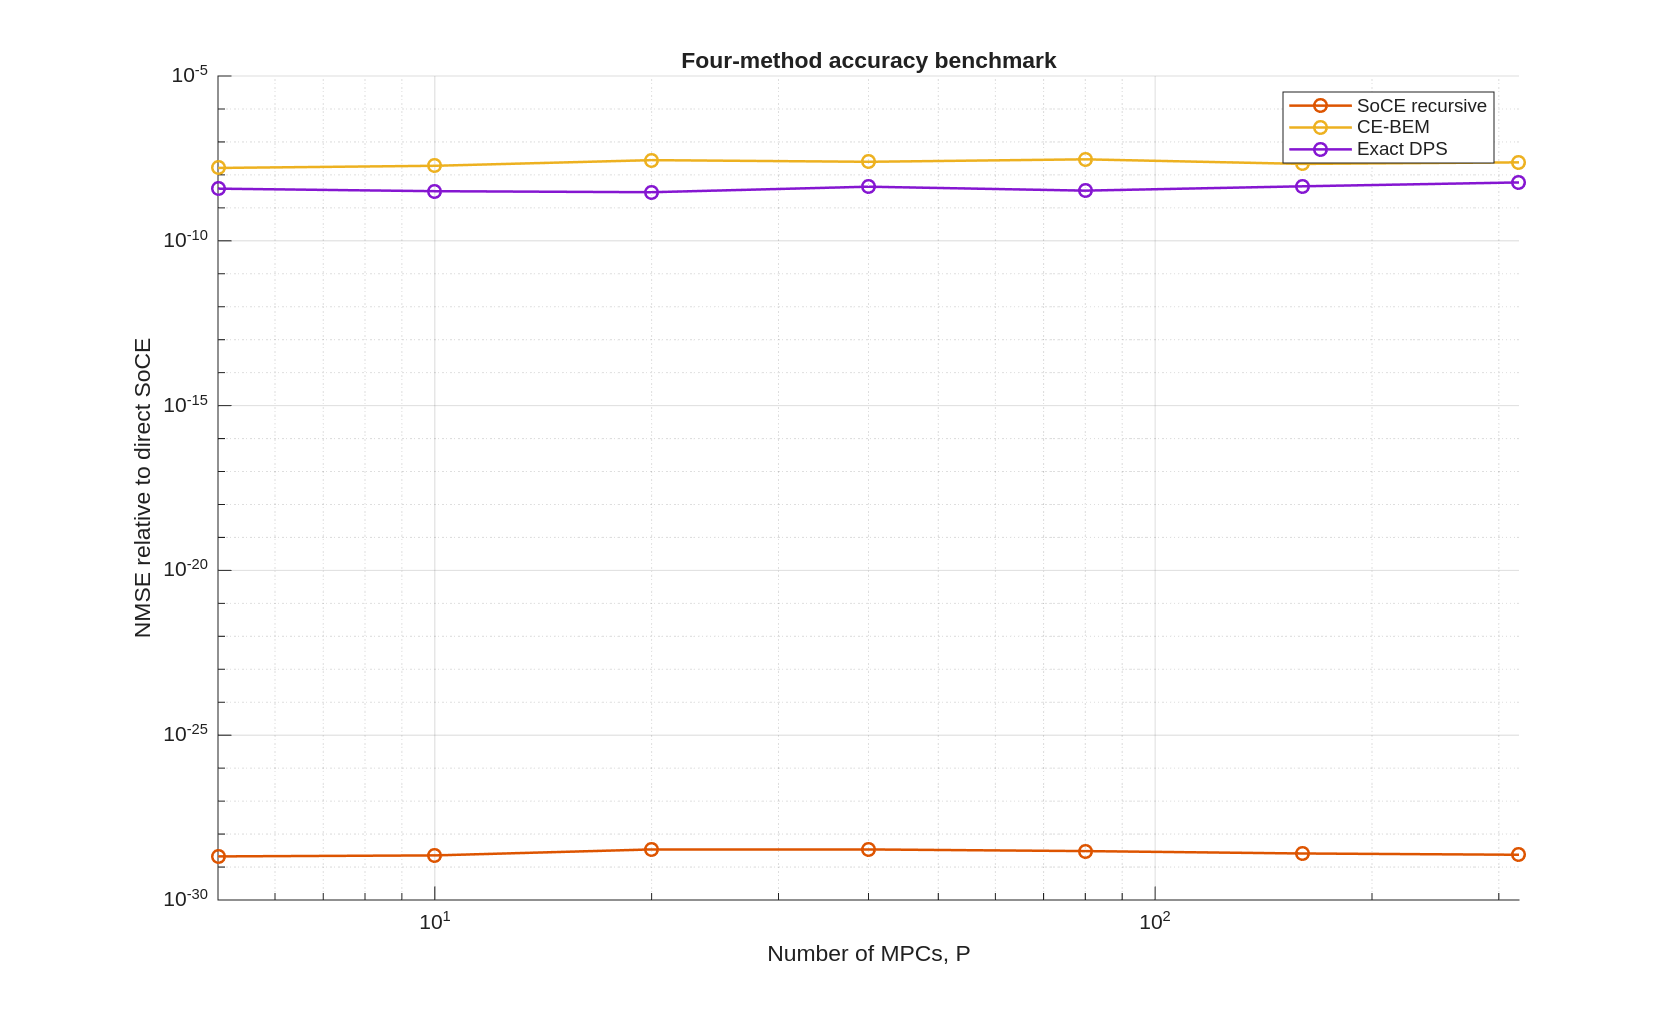
\includegraphics[width=0.9\textwidth]{results/figures/mimo_four_method_benchmark_nmse.png}
    \caption{NMSE của SoCE đệ quy, CE-BEM và DPS chính xác so với SoCE trực tiếp}
    \label{fig:ch4_four_method_nmse}
\end{figure}

Điểm hòa vốn thứ nhất được xác định theo số MPC: đó là giá trị mà thời gian xử lý mỗi khối của phương pháp đang xét chuyển từ lớn hơn sang nhỏ hơn SoCE trực tiếp và duy trì nhỏ hơn tại các điểm khảo sát tiếp theo. Trong lần đo hiện tại, CE-BEM và DPS chính xác đã nhanh hơn SoCE trực tiếp tại điểm nhỏ nhất \(P=5\) và duy trì thứ tự này đến \(P=320\). Vì sweep không chứa giá trị nhỏ hơn 5, kết quả chỉ xác định được điểm hòa vốn thực nghiệm thỏa \(P_{\mathrm{BE}}\le5\), chưa định vị chính xác giao điểm. Đối với SoCE đệ quy, chênh lệch nhỏ và khoảng tứ phân vị chồng lấn nên chưa đủ cơ sở xác lập một điểm hòa vốn ổn định.

Điểm hòa vốn thứ hai xét chi phí tiền xử lý. Thời gian tạo cơ sở đo được là \(0{,}0139\,\mathrm{s}\) cho CE-BEM và \(0{,}2264\,\mathrm{s}\) cho DPS. Tại \(P=80\), lấy chi phí tiền xử lý chia cho phần thời gian tiết kiệm trên mỗi khối cho thấy CE-BEM hòa vốn từ khối đầu tiên, còn DPS cần khoảng 6 khối. Sau ngưỡng này, cơ sở được tái sử dụng và lợi ích thời gian tích lũy theo số khối xử lý. Phân tích này giả thiết miền giới hạn băng và kích thước khối không đổi giữa các khối; nếu các tham số đó thay đổi, cơ sở phải được tạo lại và điểm hòa vốn cũng thay đổi.

Có thể biểu diễn lập luận trên dưới dạng tổng thời gian cho \(L\) khối kênh. Gọi \(T_{\mathrm{setup},a}\) là thời gian tiền xử lý và \(T_{\mathrm{block},a}\) là thời gian xử lý một khối của phương pháp \(a\). Khi cơ sở được tái sử dụng, tổng thời gian là:
\begin{equation}
T_a(L)
=T_{\mathrm{setup},a}+L T_{\mathrm{block},a}.
\label{eq:ch4_amortized_runtime}
\end{equation}
Với SoCE trực tiếp, có thể xem \(T_{\mathrm{setup,SoCE}}=0\). Nếu \(T_{\mathrm{block},a}<T_{\mathrm{block,SoCE}}\), số khối nguyên nhỏ nhất để phương pháp \(a\) không còn chậm hơn SoCE được xác định bởi:
\begin{equation}
L_{\mathrm{BE},a}
=\left\lceil
\frac{T_{\mathrm{setup},a}}
{T_{\mathrm{block,SoCE}}-T_{\mathrm{block},a}}
\right\rceil.
\label{eq:ch4_break_even_blocks}
\end{equation}
Phương trình \eqref{eq:ch4_break_even_blocks} cũng cho thấy hai trường hợp không có điểm hòa vốn hữu hạn: thời gian mỗi khối của phương pháp mới bằng hoặc lớn hơn SoCE, hoặc cơ sở phải tạo lại cho từng khối nên không thể phân bổ chi phí tiền xử lý. Do đó, điểm hòa vốn không chỉ phụ thuộc tốc độ tái tạo mà còn phụ thuộc cách hệ thống tổ chức các khối kênh và mức độ ổn định của miền giới hạn băng.

\subsection{Ý nghĩa của kết quả đối với lựa chọn phương pháp}
\label{subsec:ch4_method_selection_implications}

Các kết quả cho thấy không có một nhánh duy nhất tối ưu đồng thời cho mọi mục tiêu. Nếu ưu tiên kiểm tra độ chính xác của không gian con và chấp nhận chi phí chiếu, DPS chính xác là đối chứng phù hợp vì nó tách sai số cắt khỏi sai số xấp xỉ hệ số. Nếu ưu tiên thời gian xử lý trên cấu hình anten nhỏ đang xét, phương pháp hybrid có lợi thế thực dụng: hai chiều lớn hơn được nén bằng DPS, trong khi hai chiều không gian được giữ trực tiếp để tránh xấp xỉ không cần thiết. DPS xấp xỉ 4D vẫn hữu ích như một nhánh chẩn đoán, bởi nó cho thấy hệ quả của việc áp dụng cùng một cơ chế xấp xỉ lên tất cả các chiều mà không xét kích thước và băng thông riêng của từng chiều.

Benchmark với CE-BEM bổ sung một góc nhìn khác. Việc CE-BEM đạt thời gian thấp trong phép đo hiện tại cho thấy phần lợi ích không chỉ đến từ riêng cơ sở DPS, mà còn đến từ việc chuyển kênh sang một không gian hệ số có kích thước nhỏ. Tuy nhiên, với cùng số chiều, DPS đạt NMSE thấp hơn trong dải khảo sát. Kết quả này phù hợp với vai trò khác nhau của hai cơ sở: CE-BEM thuận lợi về cấu trúc Fourier và khả năng triển khai nhanh, còn DPS được xây dựng để tập trung năng lượng của tín hiệu giới hạn băng trên khối hữu hạn. Lựa chọn giữa chúng vì vậy cần dựa trên ngân sách sai số, khả năng dùng FFT và tần suất tái sử dụng cơ sở, thay vì chỉ dựa vào một lần đo thời gian.

Đối với một bộ mô phỏng kênh dùng nhiều lần, quy trình lựa chọn có thể bắt đầu từ miền băng và kích thước khối. Nếu tích thời gian--băng thông cho số chiều DPS gần bằng kích thước đầy đủ, SoCE hoặc CE-BEM có thể đơn giản hơn. Nếu số chiều thiết yếu nhỏ và cơ sở được dùng lại qua nhiều khối, DPS có điều kiện thuận lợi để bù chi phí tiền xử lý. Sau đó, số chiều cần được chọn theo ngưỡng sai số, và nhánh hybrid nên được xem xét khi các chiều anten quá ngắn để việc nén tiếp tục mang lại lợi ích đáng kể. Cách lựa chọn theo từng bước này phản ánh đúng bản chất đánh đổi giữa độ chính xác, thời gian và bộ nhớ đã phân tích trong đồ án.

\subsection{Giới hạn của kết quả hiện tại}
\label{subsec:ch4_limitations}

Các kết quả trong chương này vẫn có một số giới hạn. Thứ nhất, dù các sweep đã dùng 20 seed, các kết quả ở cấu hình chính và các nhánh xấp xỉ 4D vẫn dựa trên phạm vi tham số hẹp, chưa đại diện cho mọi phân bố kênh. Thứ hai, số chiều DPS và hệ số phân giải được chọn theo quy tắc hiện tại của chương trình, chưa tối ưu tự động theo một ngưỡng sai số đặt trước. Thứ ba, phép đo thời gian dùng một tập dữ liệu cố định và phụ thuộc vào môi trường thực thi, do đó chỉ nên dùng để so sánh tương đối trong cùng điều kiện đo. Benchmark bốn phương pháp đã báo riêng chi phí tạo cơ sở, nhưng chưa khảo sát trường hợp miền giới hạn băng thay đổi làm cơ sở phải được cập nhật thường xuyên.

Ngoài ra, mô phỏng hiện tại chưa khớp lại đầy đủ một hình hoặc bảng cụ thể trong bài báo Kaltenberger với toàn bộ tham số tương ứng. Vì vậy, các kết luận từ Bảng~\ref{tab:ch4_metrics} nên được diễn đạt trong phạm vi cấu hình hiện tại: DPS chính xác kiểm chứng tốt không gian con, nhánh DPS xấp xỉ 4D cho thấy ảnh hưởng của xấp xỉ hệ số, và phương pháp hybrid là lựa chọn phù hợp hơn để thảo luận cho kênh MIMO băng rộng trong mô phỏng này.

\subsection{Kết luận chương}
\label{subsec:ch4_conclusion}

Chương này đã trình bày kết quả mô phỏng và phân tích sai số, thời gian tính toán của các nhánh biểu diễn kênh. Trong cấu hình hiện tại, DPS chính xác đạt sai số nhỏ so với SoCE, cho thấy cơ sở DPS đã chọn phù hợp để kiểm chứng biểu diễn không gian con. Nhánh DPS xấp xỉ 4D có sai số lớn hơn do áp dụng xấp xỉ hệ số trên cả bốn chiều. Phương pháp hybrid đạt NMSE \(4{,}29\times10^{-7}\) so với SoCE và có thời gian tái tạo nhỏ trong lần chạy hiện tại, do đó là nhánh chính để thảo luận về mô phỏng MIMO băng rộng có độ phức tạp thấp. Benchmark bổ sung cho thấy CE-BEM và DPS chính xác đều giảm thời gian xử lý mỗi khối trong dải \(P\) đã khảo sát, trong khi DPS duy trì NMSE thấp hơn CE-BEM với cùng số chiều cơ sở trong thí nghiệm này. Phân tích điểm hòa vốn đồng thời chỉ ra rằng lợi ích thực tế còn phụ thuộc khả năng tái sử dụng chi phí tiền xử lý. Các kết quả này được tổng hợp cùng những hạn chế và hướng phát triển trong phần kết luận của đồ án.

\cleardoublepage
